

\section{OpticalElement: \textquotedbl{}MAORY\textquotedbl{}%
  \label{opticalelement-maory}%
}

\textbf{Element}: relay\_optics

\textbf{Alias}: RO

\textbf{Description}: MAORY AO relay module


\subsection{Global properties%
  \label{global-properties}%
}

\begin{quote}
\begin{alltt}
\begin{lstlisting}[frame=single]
 temperature : !ATMO.temperature
psf_filename : None
element_name : MAORY
\end{lstlisting}
\end{alltt}
\end{quote}


\subsection{Effects%
  \label{effects}%
}

Summary of Effects included in this optical element:

\setlength{\DUtablewidth}{\linewidth}
\begin{longtable*}[c]{|p{0.098\DUtablewidth}|p{0.226\DUtablewidth}|p{0.203\DUtablewidth}|p{0.110\DUtablewidth}|p{0.179\DUtablewidth}|}
\hline
\textbf{%
element
} & \textbf{%
name
} & \textbf{%
class
} & \textbf{%
included
} & \textbf{%
z\_orders
} \\
\hline
\endfirsthead
\hline
\textbf{%
element
} & \textbf{%
name
} & \textbf{%
class
} & \textbf{%
included
} & \textbf{%
z\_orders
} \\
\hline
\endhead
\multicolumn{5}{c}{\hfill ... continued on next page} \\
\endfoot
\endlastfoot

MAORY
 & 
maory\_surface\_list
 & 
SurfaceList
 & 
True
 & 
{[}20, 120, 520{]}
 \\
\hline

MAORY
 & 
maory\_generic\_psf
 & 
FieldConstantPSF
 & 
True
 & 
{[}262, 662{]}
 \\
\hline
\end{longtable*}
\label{tbl-maory}


\subsubsection{SurfaceList: \textquotedbl{}maory\_surface\_list\textquotedbl{}%
  \label{surfacelist-maory-surface-list}%
}

\textbf{Included by default}: \texttt{True}

\textbf{File Description}: list of surfaces in MAORY

\textbf{Class Description}: <no docstring>

\textbf{Changes}:

\begin{itemize}
\item 2018-11-19 (KL) Added meta data, changed Dichr. filename

\item 2019-01-28 (KL) Fixed YAML format in meta data

\item 2020-06-22 (KL) Updated file to match the MMS configuration from Carmelo

\item 2020-08-17 (KL) Pegged temperature to atmosphere

\item 2020-12-03 (KL)
\end{itemize}


\paragraph{Data%
  \label{data}%
}

\begin{figure}[H]
\noindent\makebox[\linewidth][c]{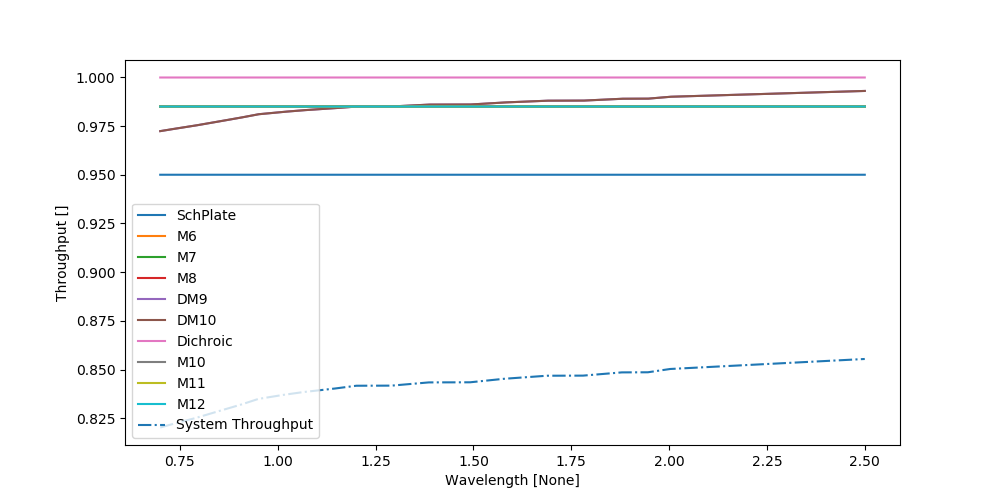
\includegraphics{maory_surface_list.png}}\phantomsection\label{fig-maory-surface-list}
\end{figure}

\setlength{\DUtablewidth}{\linewidth}
\begin{longtable*}[c]{|p{0.100\DUtablewidth}|p{0.068\DUtablewidth}|p{0.068\DUtablewidth}|p{0.068\DUtablewidth}|p{0.195\DUtablewidth}|p{0.142\DUtablewidth}|p{0.322\DUtablewidth}|}
\hline
\textbf{%
name
} & \textbf{%
outer
} & \textbf{%
inner
} & \textbf{%
angle
} & \textbf{%
temperature
} & \textbf{%
action
} & \textbf{%
filename
} \\
\hline
\endfirsthead
\hline
\textbf{%
name
} & \textbf{%
outer
} & \textbf{%
inner
} & \textbf{%
angle
} & \textbf{%
temperature
} & \textbf{%
action
} & \textbf{%
filename
} \\
\hline
\endhead
\multicolumn{7}{c}{\hfill ... continued on next page} \\
\endfoot
\endlastfoot

SchPlate
 & 
1.1
 & 
0.0
 & 
0.0
 & 
!ATMO.temperature
 & 
transmission
 & 
TER\_entrance\_window.dat
 \\
\hline

M6
 & 
1.1
 & 
0.0
 & 
0.0
 & 
!ATMO.temperature
 & 
reflection
 & 
TER\_MAORY\_mirror\_silver.dat
 \\
\hline

M7
 & 
0.7
 & 
0.0
 & 
0.0
 & 
!ATMO.temperature
 & 
reflection
 & 
TER\_MAORY\_mirror\_silver.dat
 \\
\hline

M8
 & 
0.85
 & 
0.0
 & 
0.0
 & 
!ATMO.temperature
 & 
reflection
 & 
TER\_MAORY\_mirror\_silver.dat
 \\
\hline

DM9
 & 
0.75
 & 
0.0
 & 
0.0
 & 
!ATMO.temperature
 & 
reflection
 & 
TER\_MAORY\_mirror\_mgf2agal.dat
 \\
\hline

DM10
 & 
0.75
 & 
0.0
 & 
0.0
 & 
!ATMO.temperature
 & 
reflection
 & 
TER\_MAORY\_mirror\_mgf2agal.dat
 \\
\hline

Dichroic
 & 
0.6
 & 
0.0
 & 
0.0
 & 
!ATMO.temperature
 & 
reflection
 & 
TER\_MAORY\_lgs\_dichroic.dat
 \\
\hline

M10
 & 
0.6
 & 
0.0
 & 
0.0
 & 
!ATMO.temperature
 & 
reflection
 & 
TER\_MAORY\_mirror\_silver.dat
 \\
\hline

M11
 & 
0.8
 & 
0.0
 & 
45.0
 & 
!ATMO.temperature
 & 
reflection
 & 
TER\_MAORY\_mirror\_silver.dat
 \\
\hline

M12
 & 
0.8
 & 
0.0
 & 
0.0
 & 
!ATMO.temperature
 & 
reflection
 & 
TER\_MAORY\_mirror\_silver.dat
 \\
\hline
\end{longtable*}
\label{tbl-maory-surface-list}


\paragraph{Meta-data%
  \label{meta-data}%
}

\begin{quote}
\begin{alltt}
\begin{lstlisting}[frame=single]
            filename : LIST_mirrors_maory_mms.tbl
                name : maory_surface_list
         temperature : !ATMO.temperature
        psf_filename : None
        element_name : MAORY
              author : Kieran Leschinski
              source : Carmelo Archidiacono private email
        date_created : 2018-11-19
       date_modified : 2020-06-22
              status : Design, new MAORY MMS design
          outer_unit : m
          inner_unit : m
          angle_unit : degree
    temperature_unit : deg_C
             z_order : [20, 120, 520]
             include : True
        ignore_wings : False
            wave_min : !SIM.spectral.wave_min
            wave_max : !SIM.spectral.wave_max
           wave_unit : !SIM.spectral.wave_unit
            wave_bin : !SIM.spectral.spectral_resolution
 report_plot_include : True
report_table_include : True
  minimum_throughput : !SIM.spectral.minimum_throughput
             etendue : !TEL.etendue
\end{lstlisting}
\end{alltt}
\end{quote}


\subsubsection{FieldConstantPSF: \textquotedbl{}maory\_generic\_psf\textquotedbl{}%
  \label{fieldconstantpsf-maory-generic-psf}%
}

\textbf{Included by default}: \texttt{True}

\textbf{File Description}: MAORY field varying MCAO PSF

\textbf{Class Description}: <no docstring>

\textbf{Changes}:

\begin{itemize}
\item \end{itemize}


\paragraph{Data%
  \label{id1}%
}

\begin{figure}[H]
\noindent\makebox[\linewidth][c]{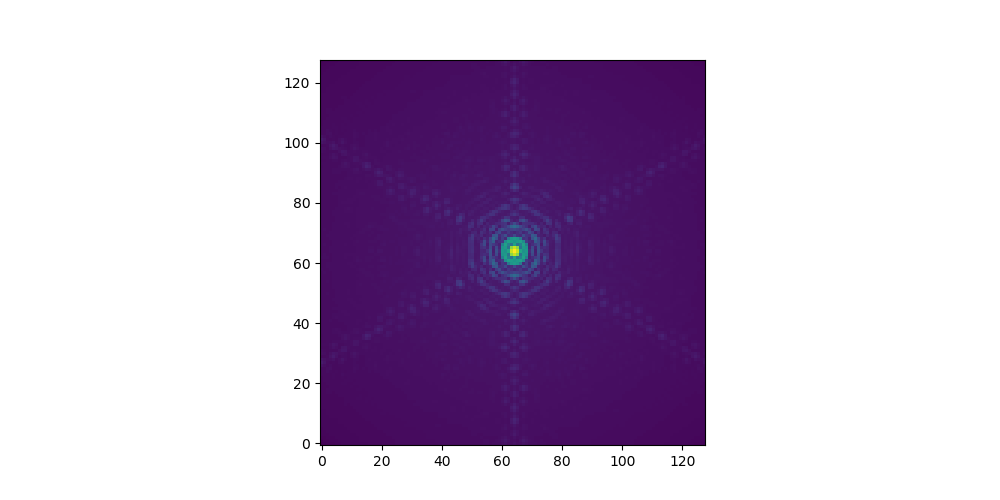
\includegraphics{maory_generic_psf.png}}\phantomsection\label{fig-maory-generic-psf}
\end{figure}


\paragraph{Meta-data%
  \label{id2}%
}

\begin{quote}
\begin{alltt}
\begin{lstlisting}[frame=single]
            filename : PSF_MCAO_ConstPSF_40_18_6.fits
                name : maory_generic_psf
         temperature : 7
        psf_filename : None
        element_name : MAORY
             warning : Default PSF is not Field Varying. See Documentation
              SIMPLE : True
              BITPIX : 8
               NAXIS : 0
              EXTEND : True
              AUTHOR : Kieran Leschinski
            DATE_CRE : 2019-07-30
            DATE_MOD : 2019-07-30
              SOURCE : AnisoCADO
              STATUS : Best guess for a MAORY ConstantPSF with AnisoCADO
               ETYPE : CONSTPSF
                ECAT : -1
               EDATA : 1
             XOFFSET : 0
             YOFFSET : 0
             z_order : [262, 662]
             include : True
       flux_accuracy : 0.001
      sub_pixel_flag : False
       convolve_mode : full
            wave_key : WAVE0
    normalise_kernel : True
 report_plot_include : True
report_table_include : False
\end{lstlisting}
\end{alltt}
\end{quote}
